\chapterpicture{header_12}
\chapter{Farmaci ansiolitici}
\markboth{Farmaci ansiolitici}{\printitle}

Il GABA è un \gamma-amminoacido, è molto importante perché coinvolge gli
stimoli inibitori, è in competizione con l'adrenalina. In opposizione al
sistema adrenergico c'è il sistema gabaergico.

Il GABA è il neurotrasmettitore che ``silenzia'' il sistema nervoso. È
il controllore inibitore del sistema nervoso.

È importante perché ci sono delle patologie legate al cervello:
\begin{itemize}
  \item Disturbi dell'ansia: comprendono fobie, disturbi del sonno
  \item Disordini d'umore
  \item Disturbi della personalità: in particolare della schizofrenia
\end{itemize}
Il GABA è un agonista del recettore GABAergico, che come azione ha un
azione di silenziamento.

In queste patologie c'è una disfunzione del GABA sul suo recettore; è
necessario intervenire facendo l'azione del GABA. Per semplificazione,
si può associare almeno un neurotrasmettitore in associazione ad alcune
patologie

Bassi livelli di GABA determinano l'insorgenza di ansia a livello
patologico.

\fullpicture*{20_001}{Stati emotivi}

L'ansia è uno stato emotivo che si ha di fronte ad una difficoltà. Non
si capisce il livello della difficoltà, ma si cerca di superarla. Un
sintomo è il battito cardiaco accelerato, sudorazione elevata, mani
fredde. In quanto ci si concentra su una parte del corpo, come un esame.
La paura è quella di non riuscire a superare un esame.

in certe situazioni però l'ansia diventa patologica, quindi si vedono
come problemi insuperabili delle situazioni che si possono superare
tranquillamente.

Le classi di farmaci che andremo a vedere sono le benzodiazepine e i barbiturici.
Per questi ultimi, un forte dosaggio porta al coma e alla morte. Sono stati soppiantati
dalle benzodiazepine, in quanto sono state scoperte per caso.

C'è un utilizzo frequente di benzodiazepine, rispetto ai barbiturici.
Rispetto ad essi sono molto più sicure, e il pericolo di morte è molto
più basso. Sono usate contro l'ansia.

Come già visto, l'ansia è diversa dalla paura. La paura ha un ostacolo
concreto, che riusciamo a razionalizzare. Mentre, l'ansia il pericolo è
incognito. In stato fisiologico sono delle emozioni che proviamo
naturalmente; possono avere una accezione fisiologica e patologica.
L'asia patologica va trattata con dei farmaci.

L'ansia è caratterizzata dal trovarsi di fronte ad uno scoglio grande, e
non ci sentiamo di avere la capacità per superare questo ostacolo.

\section{GABA}

\marginpicture*{20_002}{Acido \gamma-amminobutirrico.}

Il GABA è un neurotrasmettitore che silenzia gli stimoli. Il GABA è
l'acido \gamma-amminobutirrico. Questo neurotrasmettitore quando ha
livelli bassi, non riesce a silenziare i segnali, quindi sono accentuati
gli stati d'ansia e l'insonnia.

LA sua biosintesi è molto semplice, in quanto deve essere sintetizzato
molto velocemente. Viene sintetizzato per decarbossilaZIONE DELL' acido
glutammico. LA reazione avviene attraverso i GAD, che sono presenti
all'interno dell'SNC, ovvero dove avviene la conversione. LA conversione
deve essere rapida in quanto la soluzione ai problemi deve essere
rapida.

\begin{figure}[H]
    \centering
    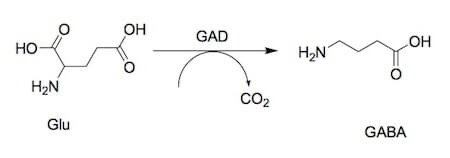
\includegraphics[width=0.7\textwidth]{20_003}
\end{figure}

Questa sintesi coinvolge la presenza di cofattori, che derivano dalla
vitamina
B\ped{6}.\ft{Un deficit di questa vitamina porta a degli scompensi come demenza o epilessia.}

La trasmissione del segnale deve avvenire in modo molto rapido. Il
recettore deve essere ionico, in quanto è molto rapido; è un canale
ionico.

I tipi di recettori per il GABA sono tre, ovvero il GABA-A e GABA-C,
ionici, e il GABA-B, che è formato da proteine accoppiate alle proteine
G.

\fullpicture*{20_004}{Tipi di recettori GABA}

Dal punto di vista farmacologico è meglio puntare su GABA-A. Il GABA-C è
presente nella retina e non viene preso in considerazione, mentre il
GABA-B è troppo lento per essere preso in considerazione

\subsection{GABA-A}

\marginpicture*{20_005}{Recettore GABA-A}

È formato da 5 subunità, due \alpha, due \beta{} e una \gamma. Nel
momento in cui il GABA si lega a questo recettore, vi è un rilascio di
ioni \ce{Cl-}, che consente di silenziare i segnali.
Lo ione cloruro (anione) è responsabile della soppressione dei segnali a
livello neuronale; gli adrenergici invece liberano cationi.

Il GABA presenta due siti di ancoraggio a livello di recettore, a
livello delle subunità \alpha{} e \beta. Per ogni recettore ci possono
essere due GABA che si legano.
Le benzodiazepine invece vanno a interagire su un sito allosterico, che
regola il recettore, potenziando.

Sono stati riconosciuti altri siti, come quello dei barbiturici,
dell'alcol (possibile) e degli steroli. In più si hanno altre parti, che
vanno ad interagire con degli antagonisti, che vengono utilizzati nel
caso sia necessario antagonizzare l'effetto del recettore. Servono a
contrastare l'effetto troppo intenso di questo recettore, come quanto
viene stimolato dai barbiturici.

Un'altra particolarità di questi recettori è che non sono tutti uguali;
sono presenti diversi tipi di subunità \alpha. Una particolare
combinazione di \alpha{} e \gamma{} porta ad avere un sito perfetto per le
benzodiazepine. Queste interagiscono con diversi recettori GABA-A, con
diversi effetti possibili. Le subunità devono essere ordinate in un
certo modo, per avere il sito allosterico.

I recettori non sono distribuiti uniformemente nel SNC, quindi non tutti
vengono modificati nello stesso momento.

Le benzodiazepine non sono né agonisti, e antagonisti, ma sono dei
modulatori del segnale. Queste hanno un attività solamente se il GABA è
presente nel sito d'azione, se il GABA è assente allora le
benzodiazepine non funzionano. Con poco GABA l'effetto diminuisce. Le
benzodiazepine modificano il gain del segnale.

Le benzodiazepine comunque sono pericolose, specialmente se miscelate ad
altro, come l'alcol. L'alcol va a interagire simultaneamente sullo
stesso recettore, quindi si modifica la risposta del recettore.

\fullpicture{20_006}{Grafico effetto vs dose per benzodiazepine e barbiturici}{fig:1}

Come si vede nel grafico \ref{fig:1}, per sopperire alle problematiche di ansia, si possono usare entrambi, i
barbiturici hanno un effetto un po' prima, quindi ne servono meno in
quanto sono più potenti.
A dosi più alte, si possono usare come anticonvulsivanti.
A dosi più alte ancora diventano degli ipnotici, in quanto si perde
coscienza di sé. Non si perde del tutto la facoltà di agire.

Le benzodiazepine, ad un certo punto, l'effetto viene fermato ad uno
stato di incoscienza (anestesia), ma non va oltre lo stato di coma e
morte. Invece i barbiturici sono più forti, e si verificano questi
effetti.
Le benzodiazepine sono utilizzate per questo motivo, in quanto sono più sicure.
Sono comunque sotto controllo medico

\marginpicture*{20_007}{Muscimolo}

Un agonista del recettore è il Muscimolo, che induce un aumento
dell'attività gabaergica. Il fungo Amanita Primaverile ha effetti
ipnotici. Causano le allucinazioni, che però sono date da un'assenza di
stimoli.
Il GABA, in una prima fase, inibisce anche sé stesso. Quindi a bassi
dosaggi, ha un effetto eccitatorio. Si ha un effetto paradosso
Il muscimolo a dosi più alte è mortale.

\marginbox*{Un allucinogeno produce un'attivazione sensoriale, mentre un ipnotico ha un effetto sedativo}

Lo stesso effetto lo fa l'alcol, che va al sito allosterico. A dosi
basse, si hanno effetti eccitatori (non al livello del muscimolo),
mentre ad alte dosi si hanno effetti inibitori. Questo comporta che si
possa arrivare al come (etilico) e anche alla morte.

\section{Benzodiazepine}

Le benzodiazepine hanno delle relazioni struttura-attività molto precise e ben note. Si sipegherà il metabolismo di
questi farmaci (come e quando devono essere somministrati) e poi si
guarderanno le caratteristiche di alcune delle benzodiazepine. Il medico
poi sceglie quale usare, però l'effetto è molto simile.

Il benzene è condensato con un ciclo diazo, la benzodiazepina
interessante dal punto di vista farmaceutico sono le 1,4 ciclo diazo.

\begin{figure}[H]
    \centering
    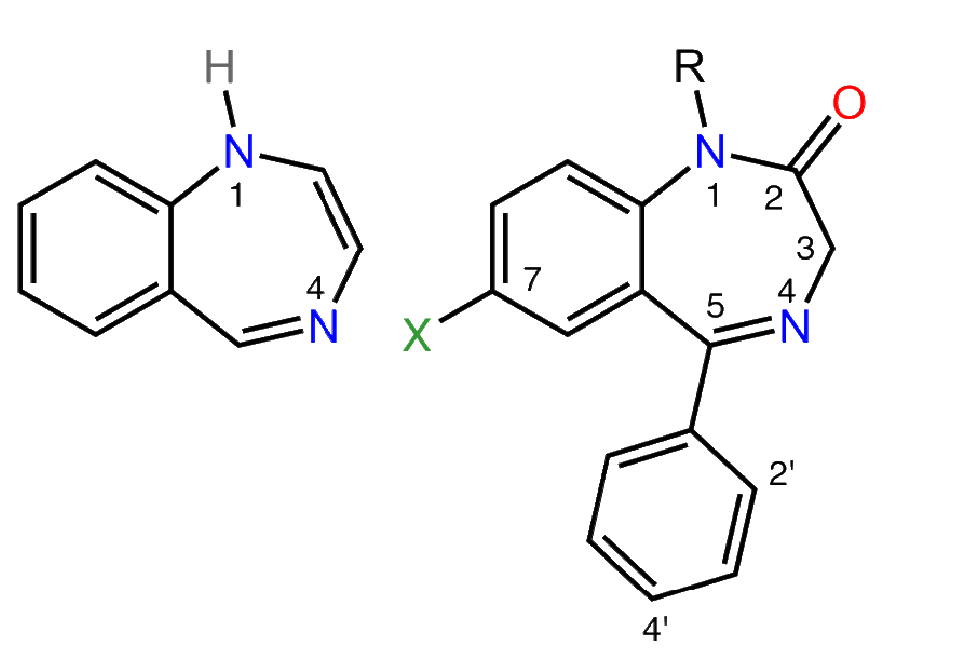
\includegraphics[width=0.6\textwidth]{20_008}
\end{figure}

È stato introdotto un lattame, ovvero un ammide ciclico come anello. La
posizione 3 non è sostituita, almeno inizialmente, però è un punto
importante nel metabolismo di queste molecole, non l'effetto
terapeutico, ma la durata dell'effetto.
Si ha poi un immina, e un fenile in posizione 5, che a sua volta può
essere sostituito in posizione 2' o 3'.
Le posizioni meta non sono utilizzate.

Una cosa che resta un mistero, è il sostituente in posizione 7, che
spesso viene aggiunto e deve essere un elettron-attrattore, per avere
una maggiore attività.

\fullpicture*{20_009}{Struttura delle benzodiazepine di prima e di seconda generazione}

Anche in questo caso si hanno due generazioni di benzodiazepine, che
migliorano dal punto di vista farmacologico, che quindi hanno una
migliore distribuzione.

Le benzodiazepine sono formate da tre anelli, che vengono nominati A, B e C.

Ci può essere anche un sostituente in posizione 3, per la prima
generazione. Questo aumenta la solubilità (da spiegare dopo).

La seconda generazione invece ha un anello a 5, che può essere un
imidazolo o un tridimazolo. A questo farmaco manca una carica. Questo
significa che queste molecole hanno bisogno di migliorare la solubilità,
quindi si è introdotto il ciclo a 5 con uno/due azoti. Questa è la
maggiore differenza tra generazione 1 e generazione 2.

Queste molecole hanno una caratteristica, che deriva dal fatto che sono
grandi e non molto idrofile. Le molecole si distribuiscono e si
accumulano nelle zone grasse, e hanno una variazione di effetto a
seconda di dove si distribuiscono. Il loro effetto è a lungo termine e
questo non è sempre voluto. Se ad esempio si prendono per andare a
dormire, sarebbe meglio prenderle subito. Anche per questo le molecole
sono state rese più polari, in quanto sono più attive e più eliminabili.
L'effetto non dovrebbe durare troppo tempo. Questo è un problema di
queste molecole.

Le benzodiazepine sono state inventate da Leo Sternbach e la prima
benzodiazepina è il Librium\footnote{The Queen's Gambit}, la molecola va
incontro a idrolisi eliminando il gruppo \ce{N-CH3}.

La scoperta è stata un caso fortuito, in quanto Sternbach stava
lavorando per la casa La-Roche, su un farmaco con effetti ansiolitici,
però non sono stati fortunati. Dopo due anni hanno smantellato il
laboratorio, però Sternbach ha notato su un becher dei cristalli, e lo
ha mandato ad un farmacologo. Non si sapeva la struttura. Quello che è
successo è che da un composto non diazepinico, se ne è formato una
benzodiazepina. Da qui si è partiti a studiare la struttura delle
benzodiazepine.

\begin{figure}[H]
    \centering
    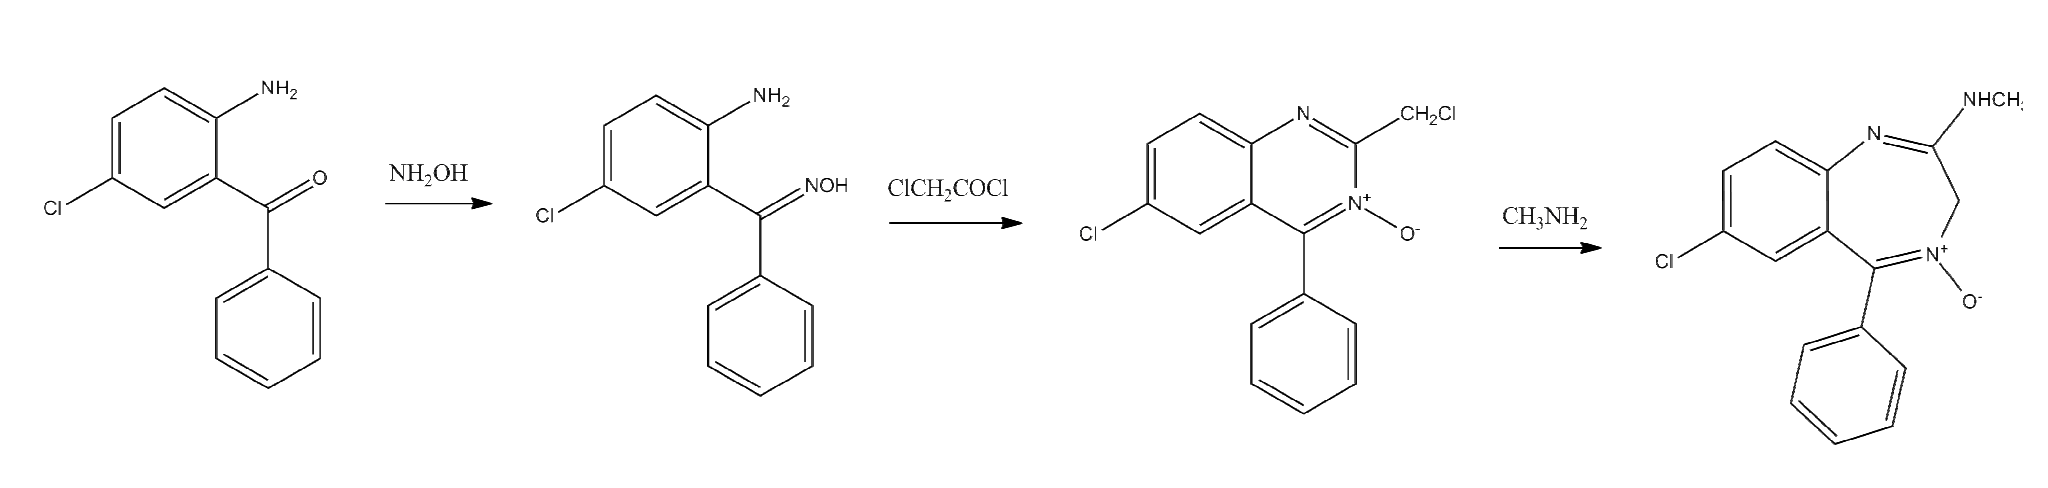
\includegraphics[width=\textwidth]{20_010}
\end{figure}

Sono riportati i farmaci che hanno la posizione 3 libera; si può mettere
un ossidrile sia dal punto della solubilità, che dal punto di vista
metabolico.

Le benzodiazepine vengono accumulate nel fegato, dove vengono
metabolizzate. Una molecola, come il diazepam, entra dentro il fegato.
In verde ci sono i gruppi che vengono modificati in modo rapido. Ad
esempio, un metile viene demetilato; il farmaco comunque è attivo. Il
farmaco assume il pre nome \emph{nor-}.

\begin{figure}[H]
    \centering
    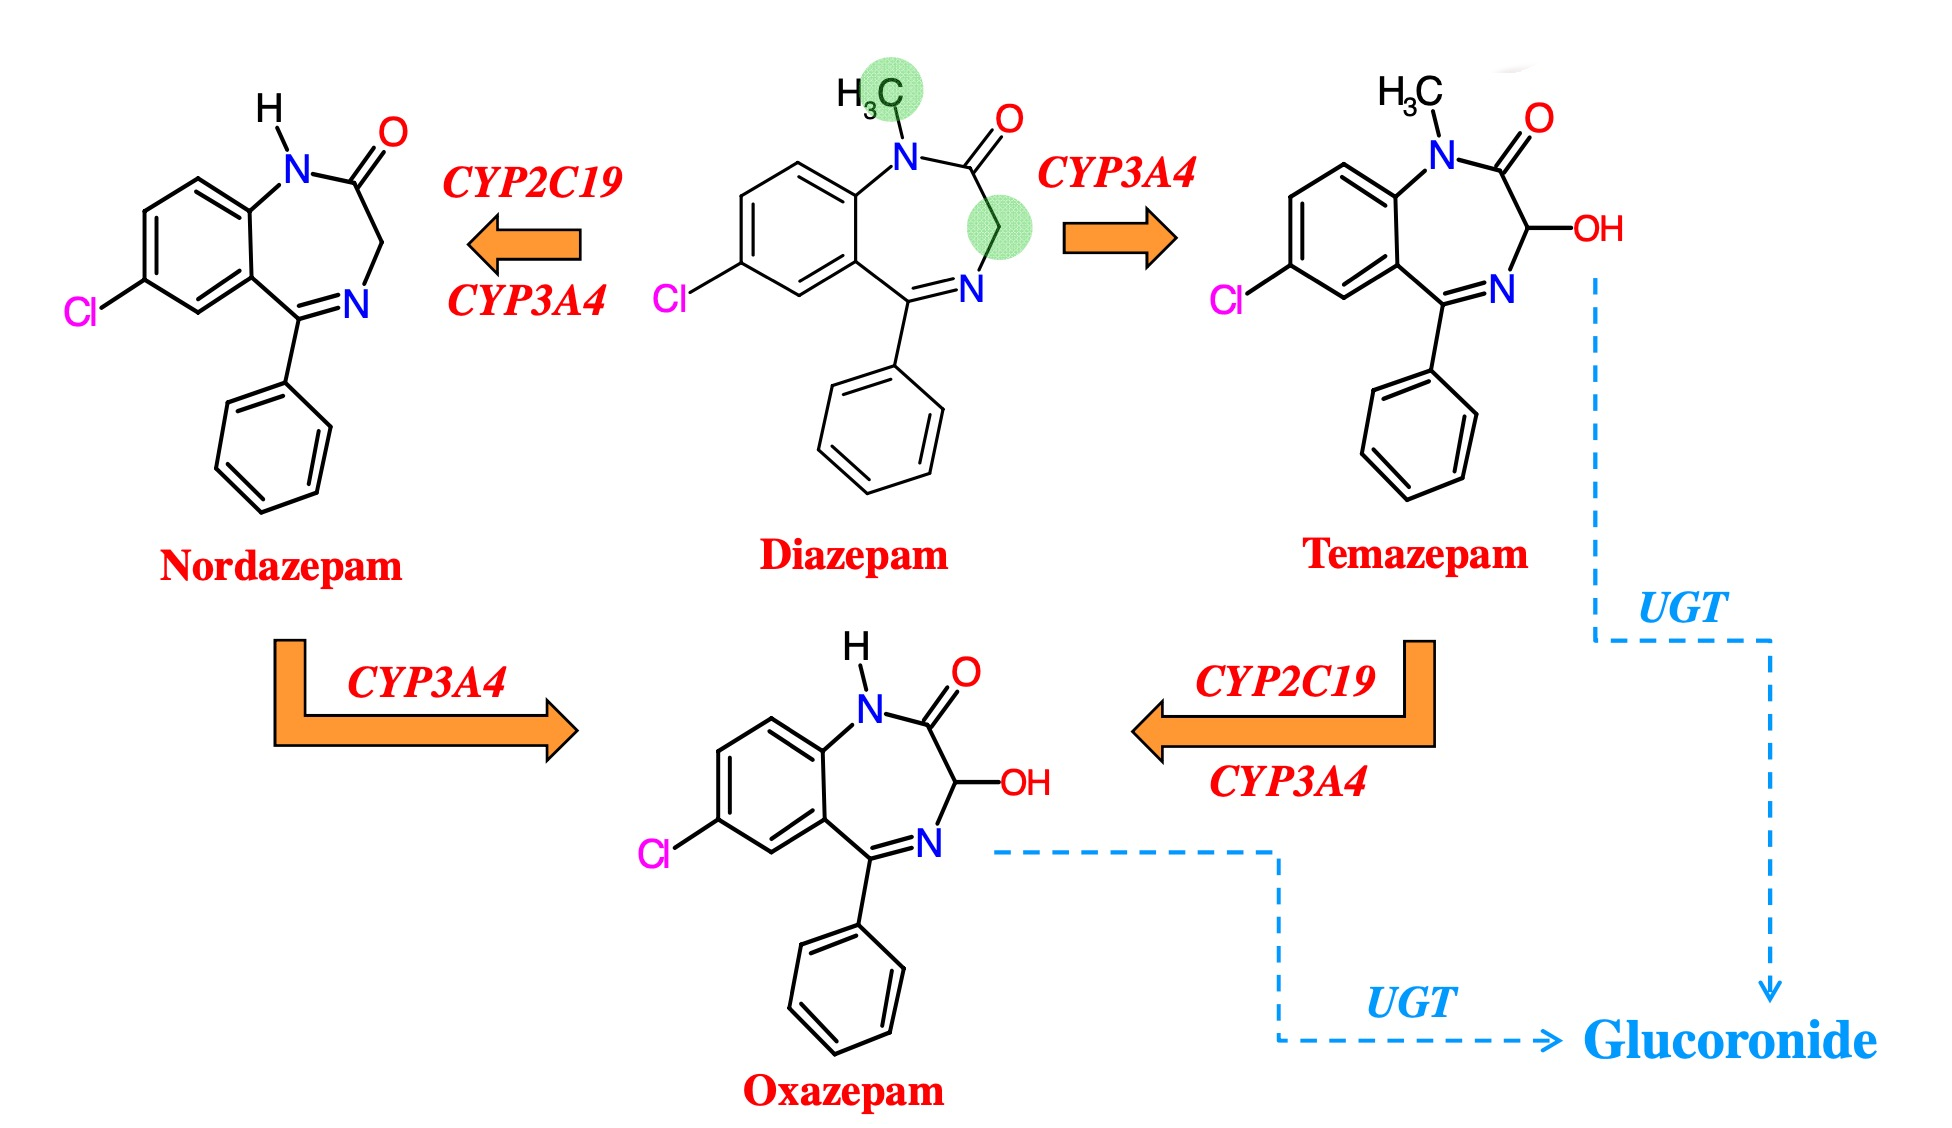
\includegraphics[width=\textwidth]{20_013}
\end{figure}

Per eliminare il farmaco, si introduce un ossidrile in posizione 3.
Quindi si forma una molecola metabolizzata, che però ha comunque un
effetto farmacologico. Il diazepam ha una vita più lunga di altri
farmaci, perché deve subire più processi per essere eliminata. Questo
serve per tarare il farmaco come durata.

Da qui i farmaci possono iniziare ad avere un ossidrile in posizione 3,
affinché durino meno.

Non si vuole che l'effetto sedativo sia troppo importante; i limiti di
effetto per le benzodiazepine sono a livello dell'ipnosi e questo si può
fare introducendo l'OH per determinare la durata, ma anche l'effetto
stesso del farmaco.

Questo tipo di molecole non danno la dipendenza caratteristica degli
oppioidi, però sviluppano una leggera tolleranza ed è
necessario smettere seguendo le prescrizioni mediche. L'effetto non è
più fisico, ma psicologico.

Nel momento in cui viene tolta bruscamente, lo stato d'ansia aumenta,
non per ragioni biochimiche. Quando si prendono questi farmaci, è
necessario seguire sempre le prescrizioni mediche.

\clearpage

\fullpicture*{20_011}{Benzodiazepine di prima generazione}

\fullpicture*{20_012}{Benzodiazepine di seconda generazione}

\clearpage

\subsection{Diazepam}

Il diazepam non ha sostituenti sull'anello C. Tutte le attività e
caratteristiche che le molecole hanno sono simili tra di loro. È un
farmaco di prima generazione.

\marginpicture*{20_014}{Struttura del diazepam}

Il $ \log{} P = 2.9$ non è basso, ma nemmeno troppo alto; queste molecole
stanno bene in zone idrofobiche e hanno una durata d'azione molto lunga,
in quanto le zone grasse servono da serbatoio per queste molecole.

L'insorgenza è di 1--1.5 ore, mentre l'emivita è di 20--100 ore. Sono lente 
ad agire e questo non è un effetto desiderato.

Se ci si aspetta l'effetto immediato, non si può fare, perché questo
genera ansia.

Una cosa svantaggiosa di questa molecola è l'emivita, che è molto
elevata. Per questo, il valium viene utilizzato per esami che
necessitano di tempo, che generano ansia ed è necessario avere i muscoli
rilassati.

L'effetto GABAergico viene usato anche per scopi non propriamente
necessari. È stato utilizzato negli USA quando è stato scoperto, sulle
casalinghe.

\marginbox*{
    Le diazepine si trovano anche in natura, ma le concentrazioni in cui
    sono presenti in patate/ciliegie non sono rilevanti a livello
    farmacologico.
}

\marginbox*{
    Il latte materno contiene un peptide GABAergico, che agisce sul
    recettore GABA-A. Il neonato, quando prende il latte materno, dorme
    meglio. Questo peptide può essere presente nel latte; questo è alla base
    del bicchiere di latte prima di dormire.
}

La pKa è riferita all'idrogeno acido in \alpha{} al gruppo carbonilico,
è stabilizzato dalle forme di risonanza.

\subsection{Clonazepam}

È un altra molecola che differisce dal diazepam molto poco; si ha
l'introduzione di un gruppo nitro. La differenza di questa molecola,è
che ha una leggera inibizione, ha una emivita dimezzata. Questa
benzodiazepina viene usata per attacchi epilettici, in quanto ha una
durata e un'intensità minore.

\marginpicture*{20_015}{Struttura del clonazepam}

Il clonazepam ha un atomo di cloro nell'altro anello, che consente di
ridurre la durata dell'azione.

\subsection{Lorazepam}

\marginpicture*{20_016}{Struttura del lorazepam}

Il lorazepam è il principio attivo del Valium. Si ha l'introduzione
dell'ossidrile, che diminuisce l'emivita di questa benzodiazepina.

\subsection{Midazolam}

\marginpicture*{20_017}{Struttura del midazolam}

È una molecola più idrofilica. Questa molecola viene metabolizzata con
un ulteriore idrossilazione al posto del gruppo metilico. Questo rende
la molecola più facilmente eliminabile.

\begin{figure}[H]
    \centering
    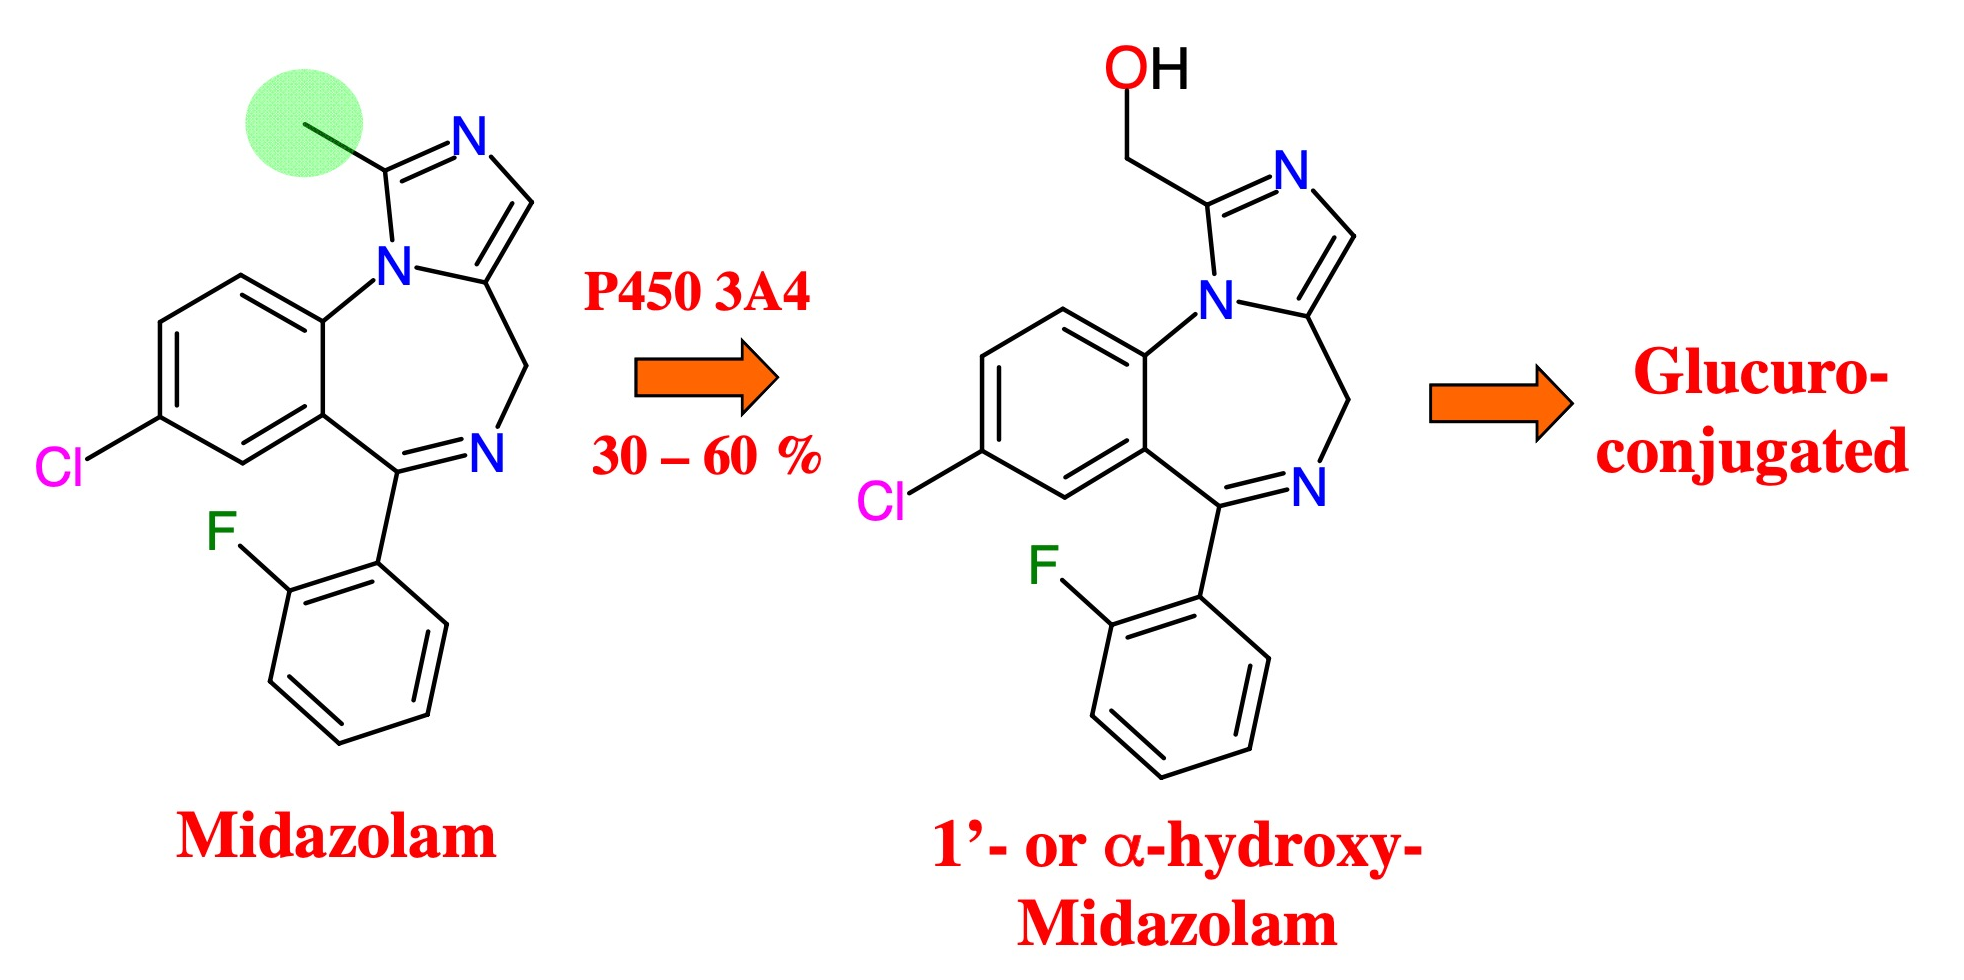
\includegraphics[width=0.75\textwidth]{20_018}
\end{figure}

\subsection{Alprazolam}

\marginpicture*{20_019}{Struttura del Alprazolam}

È lo xanax, molto utilizzato. Ha un'emivita breve, più consona per un
induttore del sonno. Ha un'emivita di 12 ore.
